\section*{Sistemas con \(N> 2\) grados de libertad}


\item
\begin{minipage}[t][2.6cm]{0.75\textwidth}
\textbf{Molécula triatómica}
Se esquematiza en la figura una molécula triatómica simétrica.
Entre dos átomos de masa $m$ hay uno de masa $M = 2 m$.
Se modelan los enlaces bajo el modelo de elasticidad de Hook con constante $k$ y longitud natural $l_0$.
\end{minipage}
\begin{minipage}[c][0cm][t]{0.2\textwidth}
  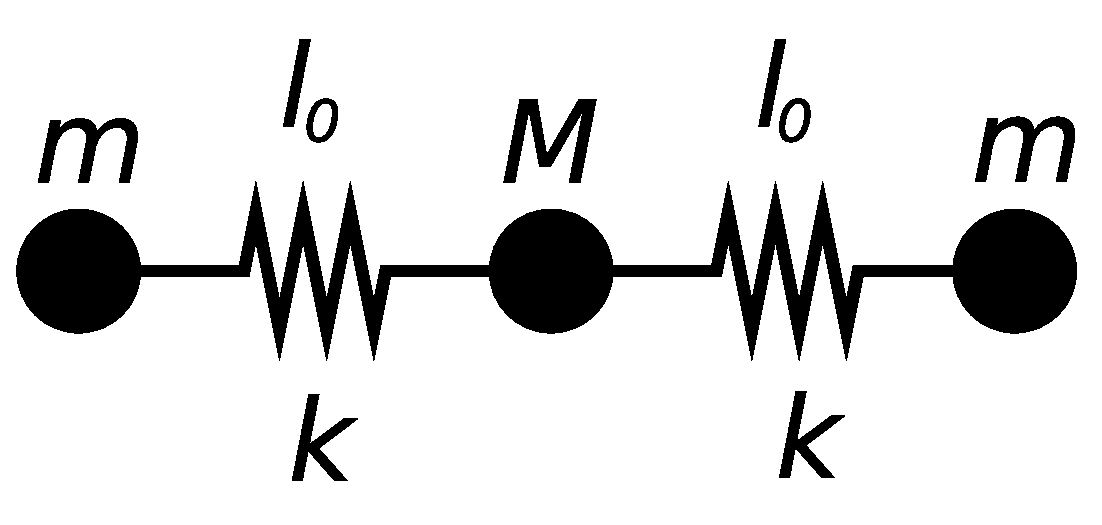
\includegraphics[width=\textwidth]{ej1-9}
\end{minipage}
\begin{enumerate}
	\item Encuentre las ecuaciones para la dinámica de cada átomo en oscilaciones longitudinales a la molécula (\(\hat{x}\)).
	Asuma que los átomos tienen impedido cualquier movimiento transversal.
	\item Halle las frecuencias de los modos normales. 
	\item Dibuje las configuraciones de cada modo. 
	\item Si el centro de masa de la molécula se mueve con $\vec{v}_0 = \mathrm{cte} \hat{x}$, escriba la solución $\vec{x}(t)$.
	\item Determine las condiciones iniciales para excitar sólo el modo de mayor frecuencia.
\end{enumerate}



\item
\begin{minipage}[t][2.2cm]{0.5\textwidth}
Analice las oscilaciones transversales del problema anterior.
Para su mejor comprensión puede imaginarlo como el esquema de la figura, en el cual las masas de los extremos pueden subir/bajar pero solidarios a la barra enhebrada a los vástagos laterales. 
\end{minipage}
\begin{minipage}[c][0cm][t]{0.45\textwidth}
  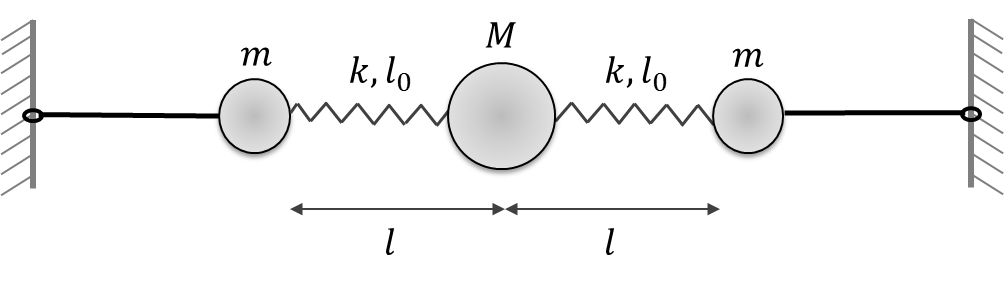
\includegraphics[width=\textwidth]{moleculaT}
\end{minipage}
\begin{enumerate}
	\item Encuentre las ecuaciones de movimiento de las masas.
	¿Qué diferencia hay en el caso con resortes \emph{slinky} y con $l_0 \neq 0$ en las ecuaciones de movimiento bajo la aproximación de pequeñas oscilaciones? 
	\item Halle las frecuencias de los modos normales.
	\item Dibuje la configuración correspondiente a cada modo normal.
Determine los desplazamientos de cada masa como función del tiempo (solución más general posible para cada masa).
	\item ¿Qué condiciones iniciales que permiten excitar sólo el segundo modo?
	\item Si se fuerza la masa del centro con frecuencias incrementalmente mayores, ¿qué modos se van observando?
	\item ¿Cómo se modifican los resultados anteriores si el extremo de la derecha se fija a la pared como se indica en la figura a continuación?.
	\begin{figure}[h]
		\centering
		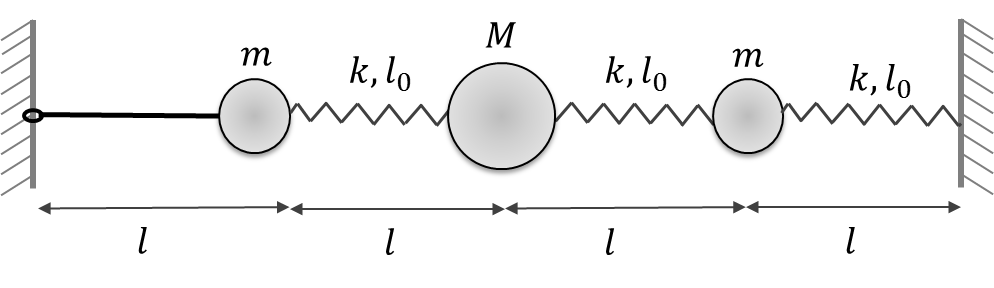
\includegraphics[clip,scale=0.5]{moleculaT_fijo_libre}
	\end{figure} 
\end{enumerate}



\item
\begin{minipage}[t][1.2cm]{0.6\textwidth}
Considere el sistema de la figura, en la que los resortes verticales tienen longitud natural $l_0$ y constante $k_1$, y los horizontales $a_0= 0$ (son ``slinkies'') y $k_2$.
Calcule las frecuencias propias y los modos normales. 
\end{minipage}
\begin{minipage}[c][1.2cm][t]{0.35\textwidth}
  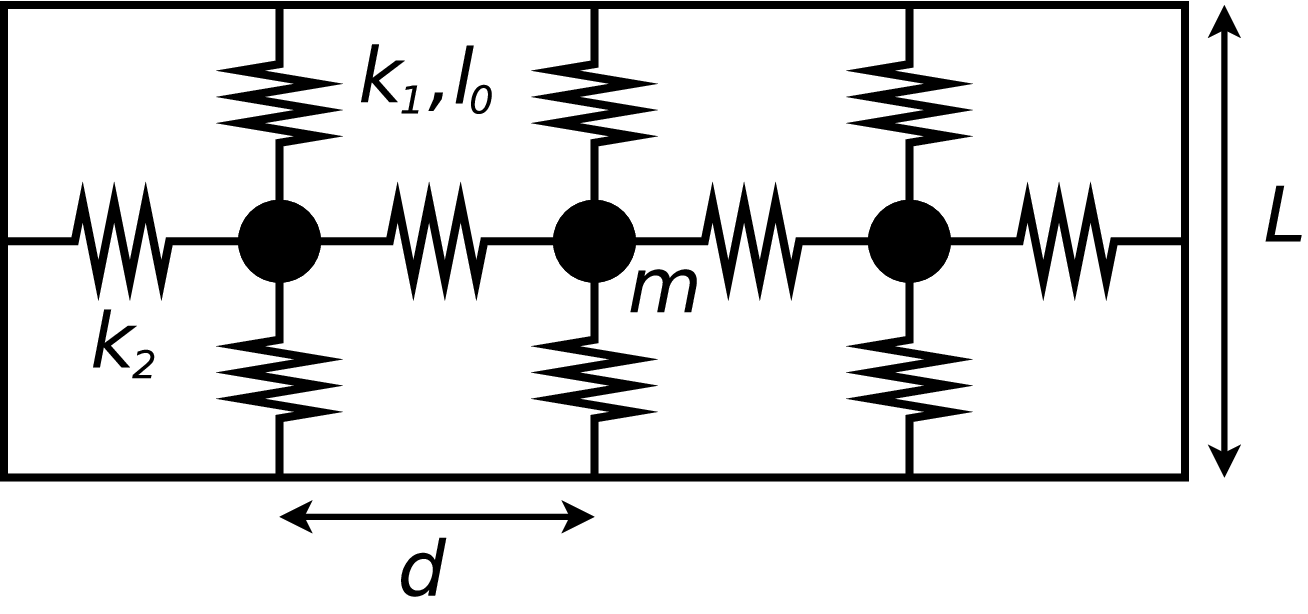
\includegraphics[width=\textwidth]{ej1-10}
\end{minipage}
